%% ============================================================================
%%  Multi-client Chat Application -- IEEE-format project report
%%  Single file: compile with  pdflatex report_ieee.tex  (run twice)
%%  Works on Overleaf (class: IEEEtran). Red text [ ... ] = fill in before submission.
%% ============================================================================
\documentclass[conference]{IEEEtran}

\usepackage[T1]{fontenc}
\usepackage{cite}
\usepackage{amsmath,amssymb}
\usepackage{graphicx}
\usepackage{xcolor}
\usepackage{booktabs}
\usepackage{array}
\usepackage{listings}
\usepackage{tikz}
\usetikzlibrary{positioning,fit,arrows.meta}
\usepackage{pgfplots}
\pgfplotsset{compat=1.16}
\usepackage[hidelinks]{hyperref}
\usepackage{balance}

% ---- helpers ---------------------------------------------------------------
\newcommand{\todo}[1]{\textcolor{red}{[#1]}}      % placeholder to fill in
\newcommand{\code}[1]{\texttt{#1}}
% contribution text under an author name: small italic, wraps inside a 1/3-page column
\newcommand{\contrib}[1]{\parbox[t]{0.30\textwidth}{\centering\footnotesize\itshape #1}}
\makeatletter
\newcommand{\linebreakand}{\end{@IEEEauthorhalign}\hfill\mbox{}\par\mbox{}\hfill\begin{@IEEEauthorhalign}}
\makeatother
\setlength{\emergencystretch}{2em}
\def\BibTeX{{\rm B\kern-.05em{\sc i\kern-.025em b}\kern-.08em T\kern-.1667em\lower.7ex\hbox{E}\kern-.125emX}}

\lstset{basicstyle=\ttfamily\scriptsize, language=Java, frame=single, framerule=0.3pt,
        backgroundcolor=\color{gray!7}, breaklines=true, columns=fullflexible,
        keywordstyle=\color{blue!60!black}, commentstyle=\color{green!40!black},
        showstringspaces=false, xleftmargin=1pt, xrightmargin=1pt, aboveskip=4pt, belowskip=2pt}

\begin{document}

% ============================================================================
%  TITLE AND AUTHORS  (5 members -- replace the red placeholders)
% ============================================================================
\title{Multi-client Chat Application: A Concurrent Client--Server System in Java with Private and Group Messaging, Persistent History and Profiling-Guided Optimization}

\author{%
\IEEEauthorblockN{Waghmode Mahesh Bapu}
\IEEEauthorblockA{
CSE, IIT Dharwad\\
cs25bt055@iitdh.ac.in\\[3pt]
\contrib{Developed the multi-threaded server, bash automation scripts and test suite.}}
\and
\IEEEauthorblockN{Pawar Shravan Mahesh}
\IEEEauthorblockA{
MnC, IIT Dharwad\\
mc25bt023@iitdh.ac.in\\[3pt]
\contrib{Client-side development: console client and its connection to the server.}}
\and
\IEEEauthorblockN{Rajiv Singh}
\IEEEauthorblockA{
CSE, IIT Dharwad\\
cs25bt036@iitdh.ac.in\\[3pt]
\contrib{GUI development: designed and built the Swing chat client.}}
\linebreakand
\IEEEauthorblockN{Adhav Shubham Balasaheb}
\IEEEauthorblockA{
MnC, IIT Dharwad\\
mc25bt020@iitdh.ac.in\\[3pt]
\contrib{Profiling: load testing, profiler and performance study.}}
\and
\IEEEauthorblockN{Divya Pratap Ade}
\IEEEauthorblockA{
CSE, IIT Dharwad\\
cs25bt048@iitdh.ac.in\\[3pt]
\contrib{Documentation: README, project report and project write-up.}}
}

\maketitle

% ============================================================================
\begin{abstract}
We built a multi-client chat application in Java. One server handles many users at the same time, and users can chat
through a console program or a window-based (GUI) program. Users register and log in with protected passwords; they can send
public, private and group messages; every message has a time stamp and is stored, so it can be read again with a history command.
Users, groups and history are kept when the server restarts. The project includes bash scripts, 20 automated tests (which found three bugs),
and a simple profiler that shows how long each part of the server takes. The profile shows that password protection is the slowest step
(by design) and that sending a message to all users costs about 2\,ms with 20 users online.
\end{abstract}

\begin{IEEEkeywords}
client--server, chat application, Java, threads, Swing, testing, profiling
\end{IEEEkeywords}

% ============================================================================
\section{Introduction}
\IEEEPARstart{C}{hat} systems are a compact but demanding example of concurrent programming: many users act at the same time,
shared data (who is online, who is in which group, what was said) must stay consistent, slow or broken clients must not harm others,
and the data must survive restarts. This project implements such a system as a client--server application, following the assignment
``develop a client--server chat application supporting multiple simultaneous users, authentication, private/group messages,
timestamps, history and server logging; GUI is optional''.

\textbf{Objectives.}
(i) Serve many users concurrently from one server;
(ii) authenticate users and store passwords safely;
(iii) support public, private and group messages with timestamps and a history command;
(iv) log server events and persist users, groups and history;
(v) provide a console client and a Swing GUI client;
(vi) automate, test and profile the system, and use the profile to improve it.

\textbf{Contributions.}
(1) a complete, working chat system in Java that uses only the standard library;
(2) a server design in which many users can chat safely at the same time;
(3) automated tests and a load generator that found three real bugs;
(4) a small built-in profiler that reports the time spent in every important method of the server, the console client and the GUI.

The rest of the paper is organized as follows. Section~II gives background, Section~III the design, Section~IV the implementation,
Section~V explains what each file of the project does, Section~VI the tools and process, Section~VII the tests, Section~VIII the profiling,
Section~IX limitations and future work, and Section~X concludes.

% ============================================================================
\section{Background and Related Work}
Text chat over TCP has a long history. Internet Relay Chat (IRC) \cite{rfc1459} defines a line-based protocol with channels
and private messages, and the Extensible Messaging and Presence Protocol (XMPP) \cite{rfc6120} streams XML between clients and servers.
Our protocol is deliberately simpler than both: one text line per command, which makes it easy to test with a plain socket.

Concurrency in Java is built on threads, monitors (\code{synchronized}), the \code{java.util.concurrent} collections and blocking queues
\cite{jcip,jdkapi}. Two server styles are common: one thread per connection (simple, used here) and event-driven non-blocking I/O
(scales to more connections but is harder to write). For password storage, current guidance recommends a slow, salted key-derivation
function such as PBKDF2 \cite{rfc8018,owasp} instead of a plain hash. A profiler measures where a program spends its time, in the same way as \code{gprof} does for C programs.

% ============================================================================
\section{System Design}

\subsection{Architecture}
Fig.~\ref{fig:arch} shows the system. Clients connect over TCP to one server process. The server contains
an accept loop, one reader thread and one writer thread per connected client, and one history-writer thread.
All reader threads share the same in-memory state and the files in the \code{data/} folder.

\begin{figure*}[!t]
\centering
\resizebox{0.86\textwidth}{!}{%
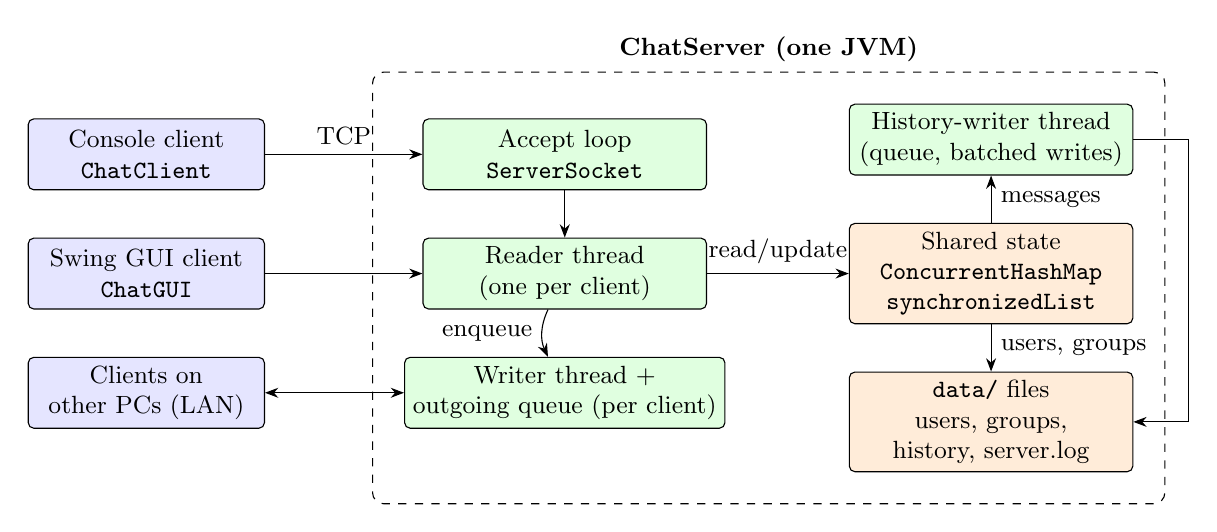
\begin{tikzpicture}[
    font=\small, >=Stealth, node distance=6mm and 14mm,
    box/.style={draw, rounded corners=2pt, align=center, minimum height=9mm, inner sep=3pt},
    cli/.style={box, fill=blue!10, minimum width=30mm},
    srv/.style={box, fill=green!12, minimum width=36mm},
    sto/.style={box, fill=orange!15, minimum width=36mm}]
  \node[cli] (con) {Console client\\\code{ChatClient}};
  \node[cli, below=of con] (gui) {Swing GUI client\\\code{ChatGUI}};
  \node[cli, below=of gui] (oth) {Clients on\\other PCs (LAN)};

  \node[srv, right=20mm of con] (acc) {Accept loop\\\code{ServerSocket}};
  \node[srv, below=of acc] (rd) {Reader thread\\(one per client)};
  \node[srv, below=of rd] (wr) {Writer thread +\\outgoing queue (per client)};

  \node[sto, right=18mm of rd] (st) {Shared state\\\code{ConcurrentHashMap}\\\code{synchronizedList}};
  \node[srv, above=of st] (hw) {History-writer thread\\(queue, batched writes)};
  \node[sto, below=of st] (fl) {\code{data/} files\\users, groups,\\history, server.log};

  \draw[->] (con.east) -- node[above] {TCP} (acc.west);
  \draw[->] (gui.east) -- (rd.west);
  \draw[<->] (oth.east) -- (wr.west);
  \draw[->] (acc) -- (rd);
  \draw[->] (rd) -- node[above] {read/update} (st);
  \draw[->] (rd) to[bend right=25] node[left, pos=.5] {enqueue} (wr);
  \draw[->] (st) -- node[right] {messages} (hw);
  \draw[->] (hw.east) -- ++(7mm,0) |- (fl.east);
  \draw[->] (st) -- node[right] {users, groups} (fl);
  \node[draw, dashed, rounded corners, inner sep=4mm, fit=(acc)(rd)(wr)(st)(hw)(fl),
        label={[font=\small\bfseries]above:ChatServer (one JVM)}] {};
\end{tikzpicture}}
\caption{System architecture: clients, server threads, shared state and persistent files.}
\label{fig:arch}
\end{figure*}

\subsection{Protocol}
The protocol is plain text, one line per message. After the connection opens, the server sends a welcome line. The client replies
\code{LOGIN <user> <pass>} or \code{REGISTER <user> <pass>} and receives \code{OK ...} or \code{ERR ...}. After login, every line is either a
command beginning with \code{/} or a public message (Table~\ref{tab:cmds}). Messages are displayed in three forms:
\code{[time] user: text} (public), \code{[time] (private) a -> b: text}, and \code{[time] [group] user: text}.
A user's history contains all public messages, only the private messages they sent or received, and only the messages of groups they belong to.

\begin{table}[!t]
\caption{Commands understood by the server}
\label{tab:cmds}
\centering\small
\begin{tabular}{@{}p{0.40\columnwidth}p{0.53\columnwidth}@{}}
\toprule
Input & Effect\\
\midrule
\code{text} & message to everyone\\
\code{/msg <user> <text>} & private message (offline users too)\\
\code{/g <group> <text>} & message to group members\\
\code{/group <cmd> <name>} & \code{cmd}: create, join, leave, members (spaces allowed, $\le$20 chars)\\
\code{/group list}, \code{/users} & list groups / online users\\
\code{/history [n]} & last $n$ visible messages (default 20, max 200)\\
\code{/help}, \code{/quit} & help, disconnect\\
\bottomrule
\end{tabular}
\end{table}

\subsection{Persistent data}
The server keeps four files in \code{data/}: \code{users.txt} (\code{name:hash}), \code{history.log} (tab-separated: time, type, sender, receiver, text),
\code{groups.txt} (\code{group:member}) and \code{server.log} (timestamped events: connections, logins, failed logins, messages, group changes, errors).
On start-up the server reloads users, groups and history. These files contain password hashes and private messages and are therefore excluded from version control.

% ============================================================================
\section{Implementation}

\subsection{Threads}
The accept loop passes every new socket to a cached thread pool (\code{Executors.newCachedThreadPool}), which runs one \code{ClientHandler}
per client. A cached pool reuses threads of departed clients and grows on demand, which suits a population that changes constantly.
Each handler also starts a writer thread (the next subsections) and the server starts one history-writer thread.

\subsection{Synchronization and collections}
Table~\ref{tab:sync} lists the shared data and how each item is protected. Explicit locks are used only where several steps must be atomic.

\begin{table}[!t]
\caption{Shared data and protection mechanism}
\label{tab:sync}
\centering\footnotesize
\begin{tabular}{@{}p{0.2\columnwidth}p{0.39\columnwidth}p{0.34\columnwidth}@{}}
\toprule
Data & Structure & Why it is safe\\
\midrule
users & {\scriptsize\code{ConcurrentHashMap}} & atomic \code{putIfAbsent}: one winner per name\\
online & {\scriptsize\code{ConcurrentHashMap}} & \code{putIfAbsent} blocks double login\\
groups & map of concurrent sets & join/leave while others send\\
history & {\scriptsize\code{synchronizedList}} & scans lock the list\\
out-lines & {\scriptsize\code{LinkedBlockingQueue}} & producer--consumer\\
files & \code{synchronized} methods & no interleaved writes; \code{groups.txt}: temp file, atomic move\\
\bottomrule
\end{tabular}
\end{table}

Three further details matter for correctness.
\emph{(a) Login ordering.} The login handler holds the client's lock while it registers the user as online and queues \code{OK}; otherwise another user's
``joined the chat'' broadcast can arrive before \code{OK} (found by the load test, Section~\ref{sec:tests}).
\emph{(b) Shutdown.} A shutdown hook places a stop marker in the history queue and waits for the writer thread, so queued messages are written when
the server is stopped with Ctrl+C or \code{kill}.
\emph{(c) Disconnect.} A \code{CountDownLatch} lets a disconnecting client wait (at most 2\,s) until its writer thread has delivered the last lines.

\subsection{Message flow}
For a public message the reader thread builds a \code{Message} with a timestamp, adds it to the history, queues its serialized form for the history-writer,
writes a log line, and puts the formatted line into the outgoing queue of every online user. Private and group messages use the same path with fewer receivers.
No thread performs file or socket I/O while holding a lock that other chat threads need (Listing~\ref{lst:store}); this keeps one slow file or one slow client from
blocking everybody else (see Section~\ref{sec:prof}).

\begin{lstlisting}[caption={Storing a message without disk I/O under a lock.},label={lst:store}]
void storeMessage(Message m) {
  synchronized (history) {   // same order in memory and file
    history.add(m);
    historyQueue.add(m.serialize());
  }
}
\end{lstlisting}

\subsection{Security}
Passwords are never stored in clear text. For each user the server draws a random 16-byte salt and stores
\code{pbkdf2\$iterations\$salt\$hash}, where the hash is PBKDF2-HMAC-SHA256 with 210\,000 iterations and a 256-bit output \cite{rfc8018}.
Login recomputes the hash and compares in constant time (\code{MessageDigest.isEqual}). Accounts created with an older unsalted SHA-256 hash are
upgraded at their next successful login. Usernames must match \code{[A-Za-z0-9\_]\{3,16\}}; group names are limited to 20 letters, digits, underscores
and spaces; tabs and newlines are removed from messages so they cannot break the history file format.

\subsection{Clients}
The \textbf{console client} runs a reader thread that prints server output and a main thread that sends typed lines. Because the server returns every
message with its timestamp, a naive client would show the sender's own message twice. On ANSI-capable terminals the client erases the typed line;
otherwise it sends \code{/echo off} and the server does not return the user's own messages.
The \textbf{Swing GUI} reads the network on a background thread and updates the window only through \code{SwingUtilities.invokeLater}.
Clicking a user or group in the side lists selects the target; a label above the input shows ``To: Everyone / bob (private) / group'',
and the GUI adds \code{/msg} or \code{/g} itself, so the input box contains only the message text. Messages are coloured by type and the lists refresh automatically.

\subsection{Course topics covered}
Table~\ref{tab:topics} maps the course topics to the project.

\begin{table}[!t]
\caption{Course topics and where they are used}
\label{tab:topics}
\centering\small
\begin{tabular}{@{}p{0.25\columnwidth}p{0.68\columnwidth}@{}}
\toprule
Topic & Use in the project\\
\midrule
Threads & thread pool; reader, writer, history-writer threads\\
Synchronization & \code{synchronized}, \code{putIfAbsent}, blocking queues, latch, shutdown hook\\
Collections & concurrent maps and sets, \code{synchronizedList}, \code{TreeSet}, queues\\
Networking & \code{ServerSocket}, \code{Socket}, text protocol, LAN use\\
File I/O & persistence, atomic file replace, batched writes\\
GUI & Swing client\\
Git, Bash, \LaTeX & branches and commits; build/test/profile scripts; this report\\
Profiling & built-in profiler and load generator\\
\bottomrule
\end{tabular}
\end{table}

% ============================================================================
\section{What Each File Does}\label{sec:files}
Table~\ref{tab:files} lists every file of the project and its job. Folders \code{bin/} (compiled classes) and \code{data/} (users, history, groups, log)
are created automatically and are not stored in Git.

\begin{table*}[!t]
\caption{Files of the project}
\label{tab:files}
\centering\small
\begin{tabular}{@{}p{0.27\textwidth}p{0.68\textwidth}@{}}
\toprule
File & What it does\\
\midrule
\code{src/ChatServer.java} & The server. Accepts connections, checks logins, delivers public, private and group messages, keeps history, saves users, groups and history in files, and writes the server log.\\
\code{src/ChatClient.java} & Console client. Connects to the server, asks for login or registration, shows incoming messages and sends what the user types.\\
\code{src/ChatGUI.java} & Window client (Swing). Login window, lists of online users and groups, click-to-choose receiver, message area, history window, buttons for groups.\\
\code{src/Prof.java} & Small profiler. Counts how often a method runs and how long it takes. Switched off unless the program is started with \code{-Dprofile=true}.\\
\code{tests/ChatTest.java} & Automatic functional tests (15 checks): registration, login, messages, groups, history, restart.\\
\code{tests/LoadTest.java} & Starts many clients that all send messages at once; checks that every message arrives and prints the speed.\\
\code{tests/SlowClient.java} & One client stops reading while another sends many messages; shows that the server keeps working.\\
\code{tests/ProfActions.java} & Uses every kind of command a few times (group create, join, leave, private message, history) so the profiler has data for them.\\
\code{scripts/run.sh} & One script to build, start the server, client or GUI, build the PDFs, or clean up.\\
\code{scripts/test.sh} & Builds the project, starts a fresh server, runs all tests, restarts the server and checks that the saved data is still correct (20 checks).\\
\code{scripts/profile.sh} & Starts the server with the profiler, runs the load test and the commands, and saves the time table in \code{docs/profiling/profile.txt}.\\
\code{sources.txt} & List of the Java files for the compiler; makes the build command the same on every operating system.\\
\code{README.md} & How to build, run, connect several PCs, test and profile.\\
\code{docs/PROFILING.md} & Step-by-step profiling guide.\\
\code{docs/report/report\_ieee.tex} & This report.\\
\code{docs/slides/slides.tex} & Presentation slides (Beamer).\\
\code{.gitignore}, \code{.gitattributes} & Tell Git which files to ignore (compiled files, user data) and to keep script line endings correct.\\
\bottomrule
\end{tabular}
\end{table*}

% ============================================================================
\section{Tools and Development Process}
\textbf{Build and automation.} Sources compile into \code{bin/} and runtime data goes to \code{data/}. Three bash scripts automate the work:
\code{scripts/run.sh} (build, start server, client or GUI, build the PDFs, clean), \code{scripts/test.sh}
(build, start a fresh server, run all tests, restart the server, check that the saved data is correct; it ends with success only if everything passes)
and \code{scripts/profile.sh} (profiling, Section~\ref{sec:prof}). Equivalent commands for Windows are given in the README.

\textbf{Version control.} \code{main} holds the working version; each task is done on a feature branch (e.g.\ \code{feature/tests-and-automation}),
committed in small steps with explanatory messages, and merged with \code{git merge --no-ff}. \code{.gitignore} excludes classes, \code{bin/}, \code{data/}
and \LaTeX{} build files. \todo{Add the output of \code{git log --oneline --graph --all} to the appendix and mention the number of commits per member.}

% ============================================================================
\section{Testing and Results}\label{sec:tests}
\code{tests/ChatTest.java} (plain Java, no external libraries) runs 15 checks, driven by \code{scripts/test.sh}:
registration with automatic login, duplicate username and wrong password rejected; public message with correct timestamp format;
private message delivered and hidden from other users; group creation with spaces in the name, non-member blocked, member receives group messages,
non-member cannot see them in history; eight threads registering the same name at once (exactly one succeeds); and, after a server restart, login,
history and group membership still intact. The script then checks that the four runtime files exist and that no password appears in clear text:
\textbf{20 of 20 checks pass}. The GUI was tested manually \todo{confirm: list what you clicked through}.

\textbf{Defects found by testing.}
(1) \emph{Groups lost after restart:} the loader accepted only names without spaces although \code{/group create} allows them.
(2) \emph{Login race:} with 50 clients joining at once, one client received another user's ``joined'' line before its own \code{OK} and its login failed;
fixed by holding the client's lock until \code{OK} is queued.
(3) \emph{Wasted hashing:} registering an existing username still computed a slow hash; the name is now checked first.

% ============================================================================
\section{Profiling}\label{sec:prof}

\subsection{How it works}
Like \code{gprof} for C, our profiler (\code{src/Prof.java}) measures the run time of each method: how many times it was called, the total time, and the average time.
Important methods of the server, the console client and the GUI are wrapped with a timer. The timers are off by default and cost almost nothing;
starting a program with \code{-Dprofile=true} turns them on, and the table is printed when the program stops.
\code{scripts/profile.sh} starts the server this way, lets 20 clients send 500 public messages each (10\,000 messages, 200\,000 deliveries),
and then runs every command type 20 times (\code{tests/ProfActions.java}). The result is saved in \code{docs/profiling/profile.txt}.
Measured time includes waiting for locks, methods call each other (a message calls \code{send} for every receiver), and users run in parallel, so rows overlap.

\subsection{Result}
Table~\ref{tab:prof} shows the most important rows of one run on a 2-core Linux machine (client programs and server on the same machine).

\begin{table}[!t]
\caption{Server profile: 20 clients $\times$ 500 messages, then 20 of each command}
\label{tab:prof}
\centering\footnotesize
\begin{tabular}{@{}p{0.43\columnwidth}rrr@{}}
\toprule
Method & Calls & Total (ms) & Avg (ms)\\
\midrule
\code{register} (with hashing) & 22 & 51\,706 & 2\,350\\
\code{publicMessage} & 10\,020 & 22\,019 & 2.20\\
\code{send} (one line to one user) & 201\,134 & 8\,348 & 0.042\\
\code{storeMessage} & 10\,060 & 3\,355 & 0.33\\
\code{login} (checks password) & 2 & 94 & 47\\
\code{/history} & 20 & 87 & 4.3\\
\code{saveUser} & 22 & 68 & 3.1\\
\code{/g} (group message) & 20 & 54 & 2.7\\
\code{/group create} & 20 & 46 & 2.3\\
\code{/msg} (private message) & 20 & 12 & 0.59\\
\code{/group join} & 20 & 5.3 & 0.26\\
\code{/users} & 20 & 1.6 & 0.08\\
\bottomrule
\end{tabular}
\end{table}

\subsection{What we learn}
\begin{itemize}
\item \textbf{Password protection is the slowest step.} Registering takes about 2.3\,s per user here because 20 users registered at once on 2 cores, and each password is hashed on purpose slowly (a single login takes about 47\,ms).
Slow hashing makes stolen password files hard to crack, so we keep it. We only avoid hashing when the user name is already taken.
\item \textbf{Normal chatting is cheap.} A public message to 20 users takes about 2.2\,ms in total; each single delivery (\code{send}) takes 0.04\,ms. The server handled about 8\,500 messages per second (170\,000 deliveries per second) in this run.
\item \textbf{Saving to files costs more than memory operations.} \code{/group create}, \code{saveUser} and \code{/history} take 2--4\,ms because they write or scan data, while \code{/group join}, \code{/users} and the other list commands take less than 0.3\,ms.
This is why the server writes the history in a background thread, and why each user has an own outgoing queue: a slow file or a slow client must not hold up everybody else.
\end{itemize}
The same method is available for the clients: for the console client it reports login time and time to send and print a line, for the GUI the time of each window update (for example \code{handleLine} and \code{appendMessage} took about 1.6\,ms and 3\,ms on average in our check). Both are very small compared with the network and server time.

\subsection{Earlier experiment and limits}
Before the final design, the first version of the server wrote the history file and every socket line while holding a lock. We compared that version with the final one
(50 clients $\times$ 1\,000 messages, three alternating runs, same 2-core machine): about 5\,183 messages per second before and 8\,650 after ($+67\%$).
In a second test one client stopped reading while another sent 20\,000 messages: with the first version the healthy receiver got only about 6\,800 of them in 20\,s, with the final version all 20\,000 in about 1\,s.
This first version is not part of the submitted code, so these two results cannot be repeated from the project files.
\emph{Limits of all numbers:} the 2-core test machine also ran the load generator, there was one kind of workload, and results vary by 10--20\% from run to run.
\todo{Run \code{scripts/profile.sh} on your own PC and replace Table~\ref{tab:prof} and the numbers in the text.}

% ============================================================================
\section{Limitations and Future Work}
\textbf{Limitations.}
(i) No encryption: messages and passwords cross the network in plain text; the password is hashed only when stored.
(ii) No limit on login attempts or line length.
(iii) The whole history is kept in memory and scanned linearly by \code{/history}.
(iv) After \code{kill -9} the few messages still queued for the history file are lost.
(v) A legitimate but very slow client that falls 10\,000 lines behind is disconnected.
(vi) One server process; the GUI has no automatic reconnect.

\textbf{Future work.} TLS (\code{SSLServerSocket}), login rate limiting and maximum line length, a database for history with an index,
message delivery acknowledgements, automatic reconnect, and file transfer.

% ============================================================================
\section{Conclusion}
We built a multi-client chat system that covers every requirement of the assignment: many users at the same time, login, private and group messages, time stamps,
history, saved data, server log and a GUI. Automated tests found three real bugs, and the profiler showed where the time goes: password protection is slow on purpose,
sending messages is fast, and file operations are the slowest parts of normal chatting. Moving file writing and slow connections out of the main message path
made the server faster and kept it working when one client stopped reading. The general lesson is to measure first and then change the design where the measurement points.

% ============================================================================
\section*{AI Usage Declaration}
In line with the course policy we declare that an AI assistant (Claude) was used for: drafting the test programs and bash scripts, proposing fixes for the
defects described in Section~\ref{sec:tests}, implementing the GUI target selection and the console echo handling, writing the load generator, the outgoing-queue redesign and the profiler,
and drafting this report and the slides. The team ran and checked the results. \todo{Each member: confirm that you understand and can explain these parts; add what you wrote or changed yourselves.}

\section*{Acknowledgment}
The authors thank \todo{instructor name} for the project guidance and the course \todo{course name}, \todo{institute}.

% ============================================================================
\balance
\begin{thebibliography}{00}
\bibitem{rfc1459} J.~Oikarinen and D.~Reed, ``Internet Relay Chat Protocol,'' RFC 1459, IETF, May 1993.
\bibitem{rfc6120} P.~Saint-Andre, ``Extensible Messaging and Presence Protocol (XMPP): Core,'' RFC 6120, IETF, Mar.\ 2011.
\bibitem{jcip} B.~Goetz, T.~Peierls, J.~Bloch, J.~Bowbeer, D.~Holmes, and D.~Lea, \emph{Java Concurrency in Practice}. Addison-Wesley, 2006.
\bibitem{jdkapi} Oracle, ``Java Platform, Standard Edition API Specification: \texttt{java.util.concurrent}, \texttt{java.net}, \texttt{javax.swing}.''
\bibitem{rfc8018} K.~Moriarty, B.~Kaliski, and A.~Rusch, ``PKCS \#5: Password-Based Cryptography Specification Version 2.1,'' RFC 8018, IETF, Jan.\ 2017.
\bibitem{owasp} OWASP Foundation, ``Password Storage Cheat Sheet.''
\end{thebibliography}

\end{document}
